\documentclass[11pt]{article}
\newcommand{\numpy}{{\tt numpy}}    % tt font for numpy
\newcommand{\scipy}{{\tt scipy}}            % tt font for scipy
\newcommand{\matplotlib}{{\tt matplotlib}}  % tt font for matplotlib

\usepackage{amssymb,amsmath}
\usepackage{graphicx}

\usepackage[margin=.9in]{geometry}
\usepackage{hyperref}
\hypersetup{
    colorlinks=true,
    linkcolor=cyan,
    filecolor=magenta,      
    urlcolor=blue,
}

\begin{document}

$$\mbox{\Large \textbf {CS 111 (S19): Homework 7}}$$
$$\mbox{\textbf {Due by 6:00 PM, Wednesday, June 5}}$$
$$\mbox{\textbf {NAME and PERM ID No.:} Chen Li, 5468137 (replace with yours)}$$
$$\mbox{\textbf {UCSB EMAIL:} chenli@ucsb.edu (replace with yours)}$$

\par\bigskip
{\bf 1.} (Compare NCM problem 1.38.)
The moral of this problem is that, with floating-point arithmetic,
sometimes two algorithms look equivalent but one is better than the other
at getting an accurate answer.
Suppose you have a number $\hat x$ that is an approximation to another number $x$.
Define the {\em relative error} in $\hat x$ as 
$|(\hat x - x) / x |$.
(This only makes sense if $x\ne0$.)

\par\medskip
{\bf 1a.}
The classic quadratic formula says that the two roots of the quadratic equation
$$ ax^2 + bx + c = 0$$
are
$$ x_0, x_1 = \frac{-b\pm\sqrt{b^2-4ac}}{2a}. $$
Use this formula in \numpy\ (show your input and output) to compute both roots for
$$ a = 1, \;\; b = \mbox{10,000,000,000}, \;\; c = 1. $$
Also compute the roots two other ways: 
first with \numpy's {\tt np.roots()}, and then by hand.
To at least one significant digit, what is the relative error of the 
approximation computed using the quadratic formula to $x_0$? To $x_1$?
What are the relative errors of the approximations computed using {\tt np.roots()}?\\
\\For by hand, $x^2+10^{10}x+1=0$ is equivalent to $(x+10^{10}-10^{-10})(x+10^{-10})=-10^{-20}$, so solution is $-10^{10}$ and $-10^{-10}$\\
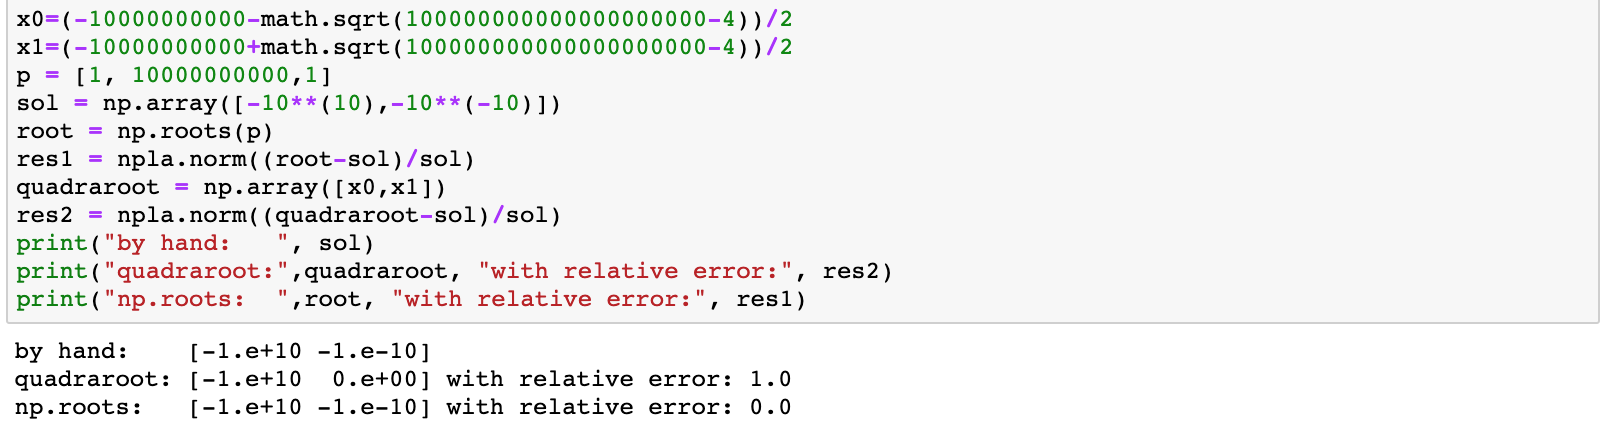
\includegraphics[scale = 0.6]{1a}
\par\medskip
{\bf 1b.}
You should have found in (1a) that the classic formula is good for 
computing one root but not the other. 
Explain in a sentence why in this case one root isn't computed accurately.
Hint: The answer involves IEEE floating-point arithmetic!\\\\
the reason is that the exponent part are large because it need to store $10^{10}$, this make the exponent of the last digit of mantissa(gap size), which is the deciding factor of accuracy large. Therefore, when such two very large number with relatively very small difference make subtraction, the result is relative too small comparing with gap size and lead to lack of accuracy.

\par\medskip
{\bf 1c.}
Use the classic formula to compute one root accurately, and then use the
fact that
$$ x_0x_1 = \frac{c}{a} $$
to compute the other.
What are the relative errors now?\\\\
$x_0 = -1.e+10,$ thus, $x_1 = $\\
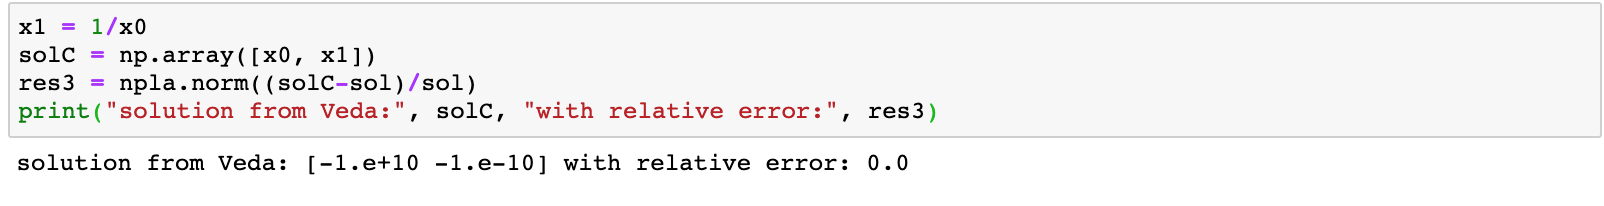
\includegraphics{1c.png}

\par\bigskip
{\bf 2.}
The standard form of a first-order ODE initial value problem is
$$ \dot y = f(t, y), \;\; y(t0) = y0, $$
where $t$ is a scalar and $y$ is a vector.
Write each of the following ODEs as an equivalent first-order system
of ODEs in standard form:

\par\bigskip
{\bf 2a.} Van der Pol equation:
$$ \frac{d^2 x}{dt^2} = (1-x^2)\frac{dx}{dt} - x . $$
$$y = x'$$ 
$$y'=x''=(1-x^2)y-x$$
$$\left(
   \begin{array}{c}
      x' \\ 	
      y' \\ 	
   \end{array} \right)=
   \left(
   \begin{array}{cc}
      0&1 \\ 	
      -1&1-x^2 \\ 	
   \end{array} \right)
   \left(
   \begin{array}{c}
      x \\ 	
      y\\ 	
   \end{array} \right)$$

\par\bigskip
{\bf 2b.} Blasius equation:
$$ \frac{d^3 x}{dt^3} = -x\frac{dx}{dt}. $$
$$x_1 = x'$$ 
$$x_2 = x_1'$$
$$x_3=x_2'=-xx_1$$
$$\left(
   \begin{array}{c}
      x' \\ 	
      x_1' \\
      x_2' 	
   \end{array} \right)=
   \left(
   \begin{array}{ccc}
      0&1&0 \\ 	
      0&0&1 \\
      0&-x&0 	
   \end{array} \right)
   \left(
   \begin{array}{c}
      x \\ 	
      x_1\\
      x_2 	
   \end{array} \right)$$

\par\bigskip
{\bf 2c.} Newton's second law of motion for a two-body problem in 2 dimensions 
($G$ and $M$ are constants):
\begin{align}
\frac{d^2 x_0}{dt^2} &= -GM\frac{x_0}{(x_0^2 + x_1^2)^{3/2}}, \\
\frac{d^2 x_1}{dt^2} &= -GM\frac{x_1}{(x_0^2 + x_1^2)^{3/2}}.
\end{align}
$$\left(
   \begin{array}{c}
      x_0'\\ 	
      x_0''\\
       	x_1'\\x_1''
   \end{array} \right)=
   \left(
   \begin{array}{cccc}
      0&1&0&0 \\ 	
      \frac{-GM}{(x_0^2+x_1^2)^{\frac{3}{2}}}&0 	&0&0\\
      0&0&0&1\\
      0&0&\frac{-GM}{(x_0^2+x_1^2)^{\frac{3}{2}}}&1
   \end{array} \right)
   \left(
   \begin{array}{c}
      x_0\\ 	
      x_0'\\ x_1 \\	x_1'
   \end{array} \right)$$

\par\bigskip
{\bf 3.} (Compare NCM problem 7.16.)
This problem is partly about ODEs and partly about making nice plots with
\matplotlib\ (we import {\tt matplotlib.pyplot} as {\tt plt}).

Many modifications of the Lotka--Volterra predator-prey model
that we saw in class have been proposed to
more accurately reflect what happens in nature.
For example, the number of rabbits can be prevented from growing
indefinitely by fixing a maximum number $R$ and changing the equations to
\begin{align}
\frac{dr}{dt} &= 2\Big(1-\frac{r}{R}\Big)r - \alpha rf, \\
\frac{df}{dt} &= -f + \alpha rf,
\end{align}
where $t$ is time, $r(t)$ is the number of rabbits, 
$f(t)$ is the number of foxes, and $\alpha>0$ is a constant.
This makes $dr/dt$ negative whenever $r > R$, 
which guarantees that the number of rabbits can never grow to exceed $R$.

For $\alpha = 0.01$, compare the behavior of the original model
with the behavior of this modified model with $R = 400$.
Solve the equations (using {\tt integrate.solve\_ivp()} as we did in class)
over 50 units of time, 
assuming that there are initially 300 rabbits and 150 foxes.
Make four different plots to show the solutions and the phase
space diagrams for both models as follows:
\begin{itemize}
\item number of foxes and rabbits (on the same plot) versus time for the original model,
\item number of foxes and rabbits (on the same plot) versus time for the modified model,
\item number of foxes versus number of rabbits (phase space) for the original model,
\item number of foxes versus number of rabbits (phase space) for the modified model.
\end{itemize}
For all plots, label all curves (with {\tt plt.legend()}) and all axes,
and put a title on each plot that identifies it clearly.
For the phase space plots, set the aspect
ratio so that equal increments on the $x$- and $y$-axes are equal in size.
(You may find the \matplotlib\ tutorial linked under the ``help'' menu
in Jupyter useful.)\\
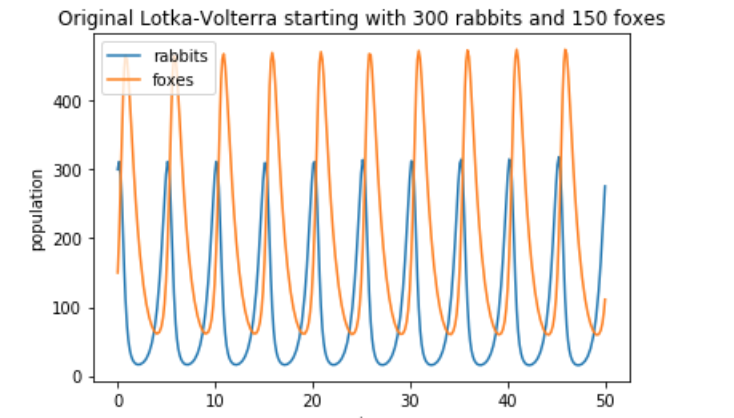
\includegraphics[scale = 0.65]{31}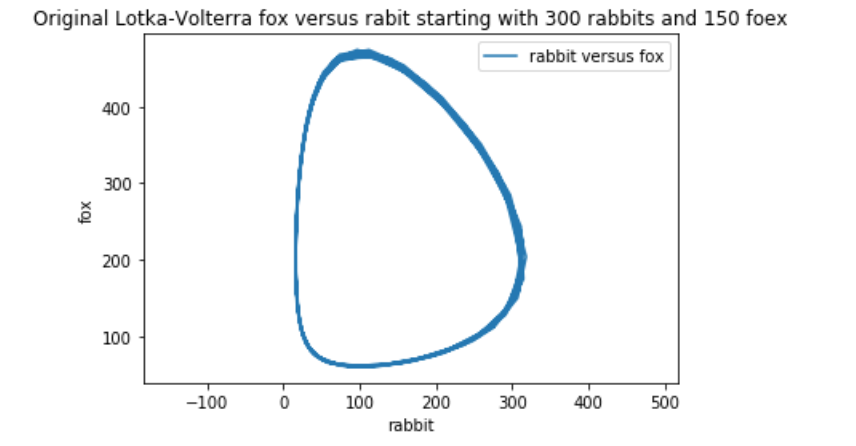
\includegraphics[scale = 0.65]{32.png}\\
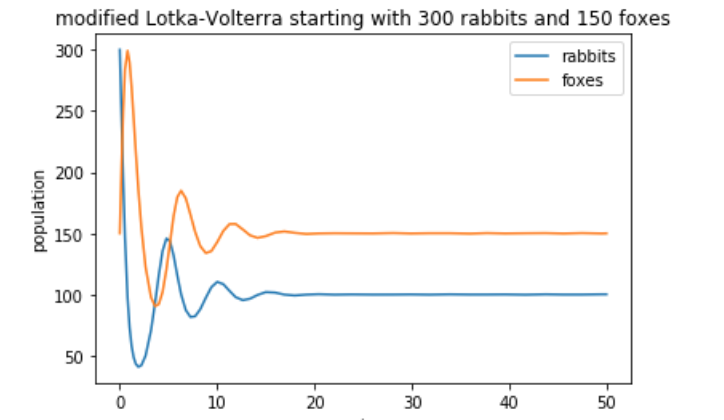
\includegraphics[scale = 0.65]{33.png}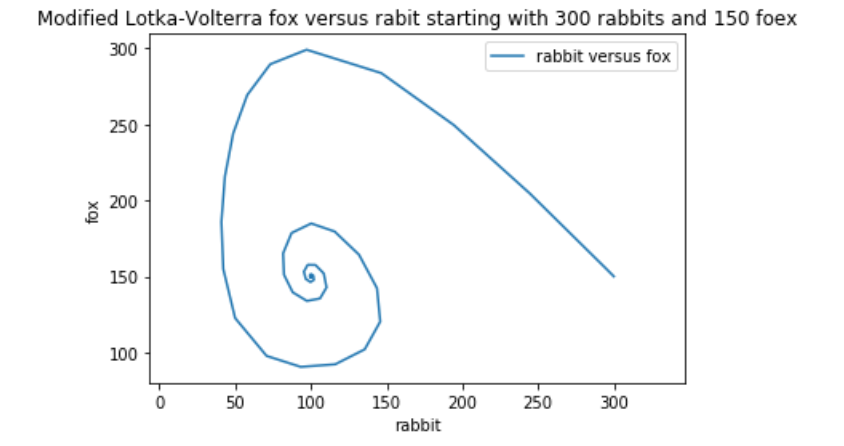
\includegraphics[scale = 0.65]{34.png}

\newpage
{\bf 4.} 
An important problem in classical mechanics is to determine the motion
of two bodies under mutual gravitational attraction.
Suppose that a body of mass $m$ is orbiting a second body of much larger mass $M$,
such as the earth orbiting the sun.
From Newton's laws of motion and gravitation,
the orbital trajectory $(x_0(t), x_1(t))$ is described by the system
of second-order ODEs
\begin{align}
\ddot x_0 &= -GMx_0/r^3, \\
\ddot x_1 &= -GMx_1/r^3, 
\end{align}
where $G$ is the gravitational constant and $r = (x_0^2 + x_1^2)^{1/2} = ||x||$
is the distance of the orbiting body from the center of mass of the two bodies.
For this exercise, we choose units such that $GM=1$.

\par\medskip
Use {\tt integrate.solve\_ivp()} to solve this system of ODEs with the initial conditions
\begin{align}
x_0(0)      = 1-e, & \;\;\; x_1(0)      = 0, \\
\dot x_0(0) = 0,   & \;\;\; \dot x_1(0) = \Big(\frac{1+e}{1-e}\Big)^{1/2},
\end{align}
where $e$ is the eccentricity of the resulting elliptical orbit,
which has period $2\pi$.
Try the values $e=0$ (which should give a circular orbit),
$e=0.5$, and $e=0.9$.
For each case, solve the ODE for at least one orbital period and obtain output 
at enough intermediate points to draw a smooth plot of the orbital trajectory.
Make separate plots of $x_0$ versus $t$, $x_1$ versus $t$, and $x_0$ versus $x_1$,
all with well-labeled axes and clear titles.
For your plot of the orbit itself, $x_0$ versus  $x_1$, 
use {\tt plt.gca().axis('equal')} to make sure the scale is the same on both axes,
so that a circle will look like a circle.\newpage
All the plot are drawn  with $5*2\pi$ time.\\
When e = 0:\\
$$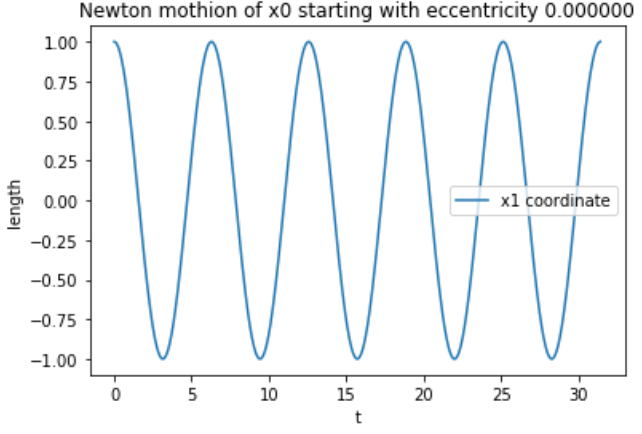
\includegraphics[scale = 0.8]{413.png}\\$$
$$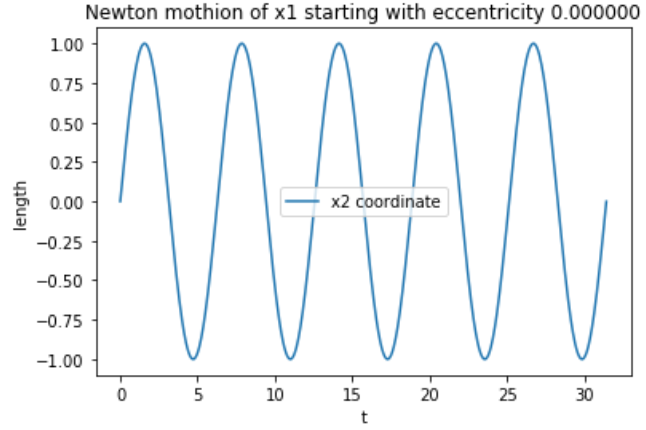
\includegraphics[scale = 0.8]{412.png}\\$$
$$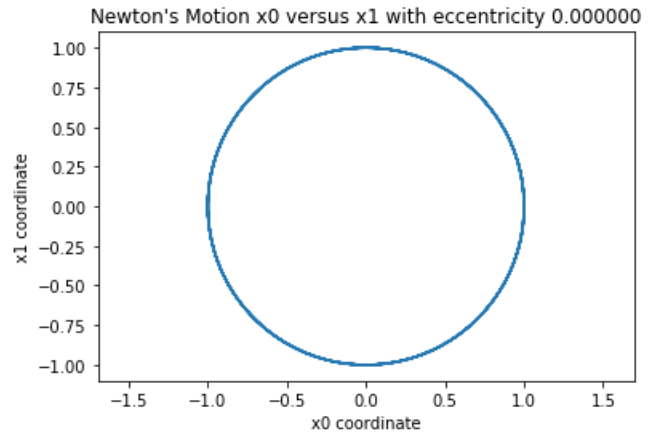
\includegraphics[scale = 0.8]{411.png}$$\newpage
when e = 0.5:
$$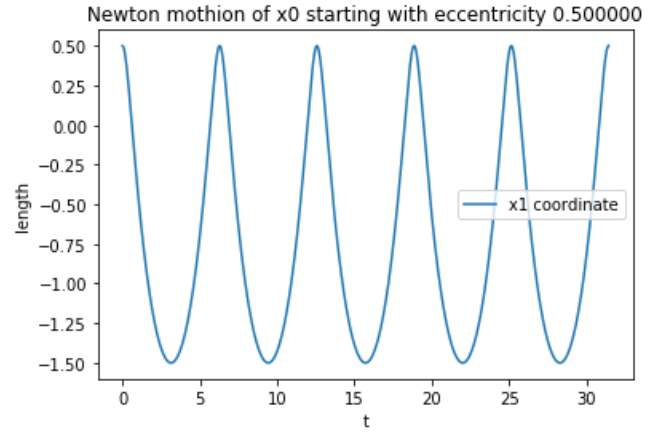
\includegraphics[scale = 0.8]{421.png}\\$$
$$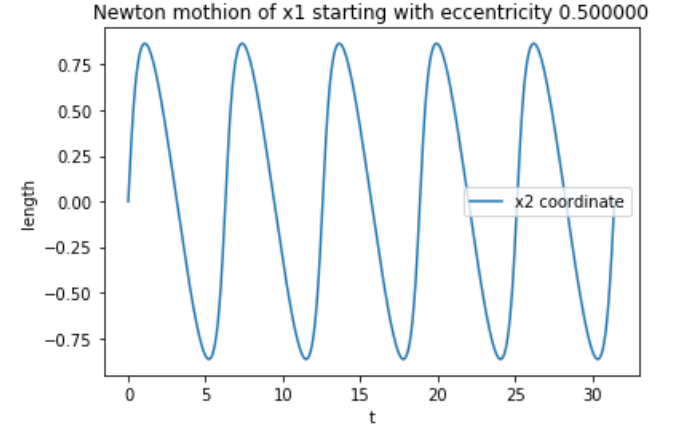
\includegraphics[scale = 0.8]{422.png}\\$$
$$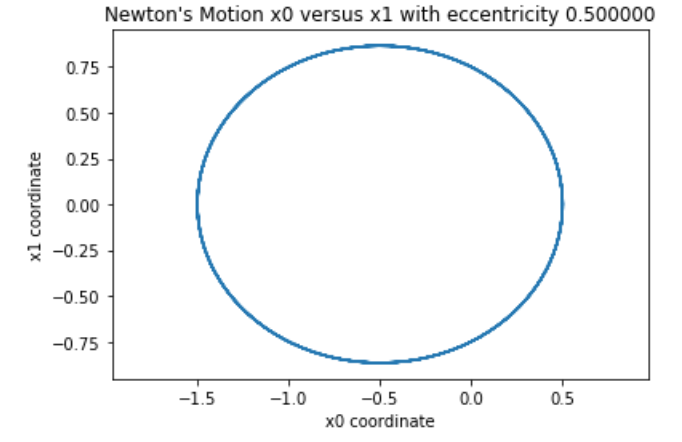
\includegraphics[scale = 0.8]{423.png}$$\newpage
when e = 0.9:
$$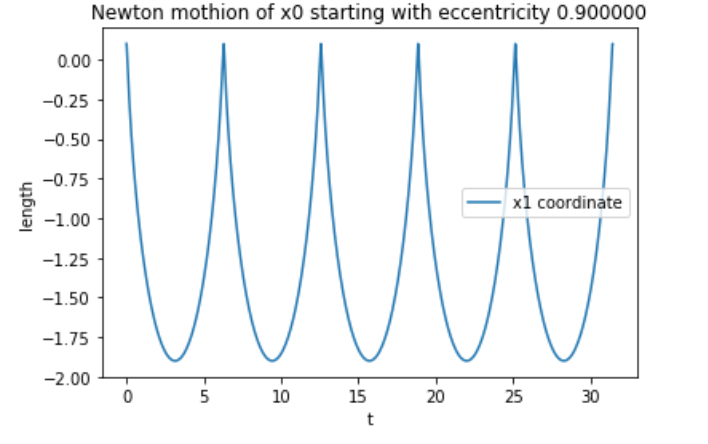
\includegraphics[scale = 0.8]{431.png}\\$$
$$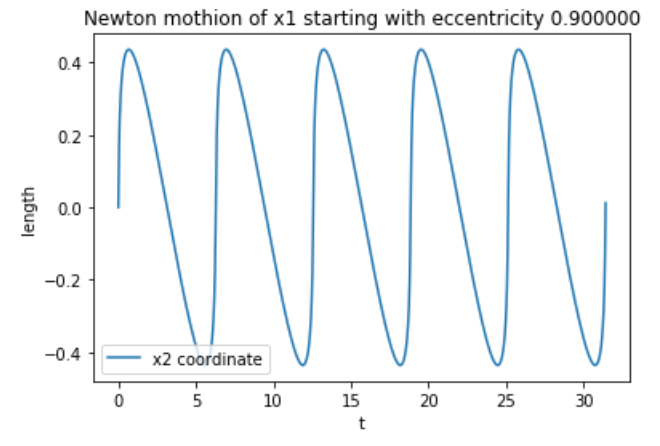
\includegraphics[scale = 0.8]{432.png}\\$$
$$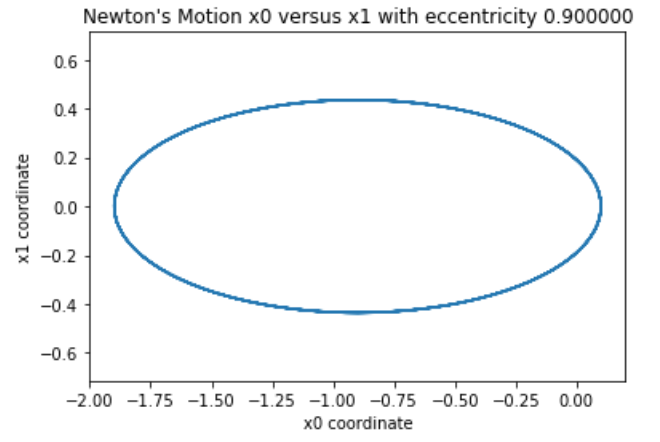
\includegraphics[scale = 0.8]{433.png}$$\newpage

\newpage

Experiment with different error tolerances 
(use {\tt help(integrate.solve\_ivp)} to find out how to set error tolerances)
to see how they affect 
(i)  the amount of time required for the solution and 
(ii) how close the orbit comes to being closed.
If you trace the orbit through several periods, 
does the orbit tend to wander or remain steady?
\par
In addition to your plots, 
turn in an explanation in English of what experiments you did,
what you observed, and what your conclusions were.\\
\\Here is a code for experiment, the trajectory of 100 period will be plot in blue line, the starting point will be plot as an orange point and the end point at 100 period will be plot as a green point. Based on math, these two points is supposed to be overlapped. Therefore, we can visualize the deviation of the stimulation by the shape of trajectory and the distance of starting and end point. For accuracy, eccentricity were set to 0.99\\
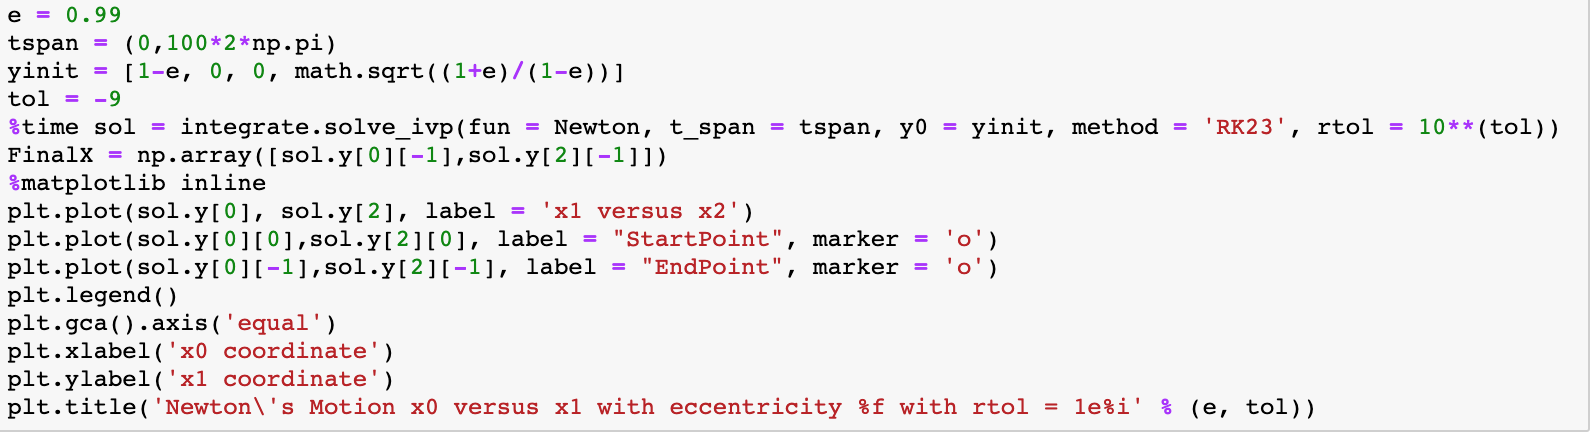
\includegraphics[scale = 0.6]{lab}\\
tol = -3, extremely inaccurate\\
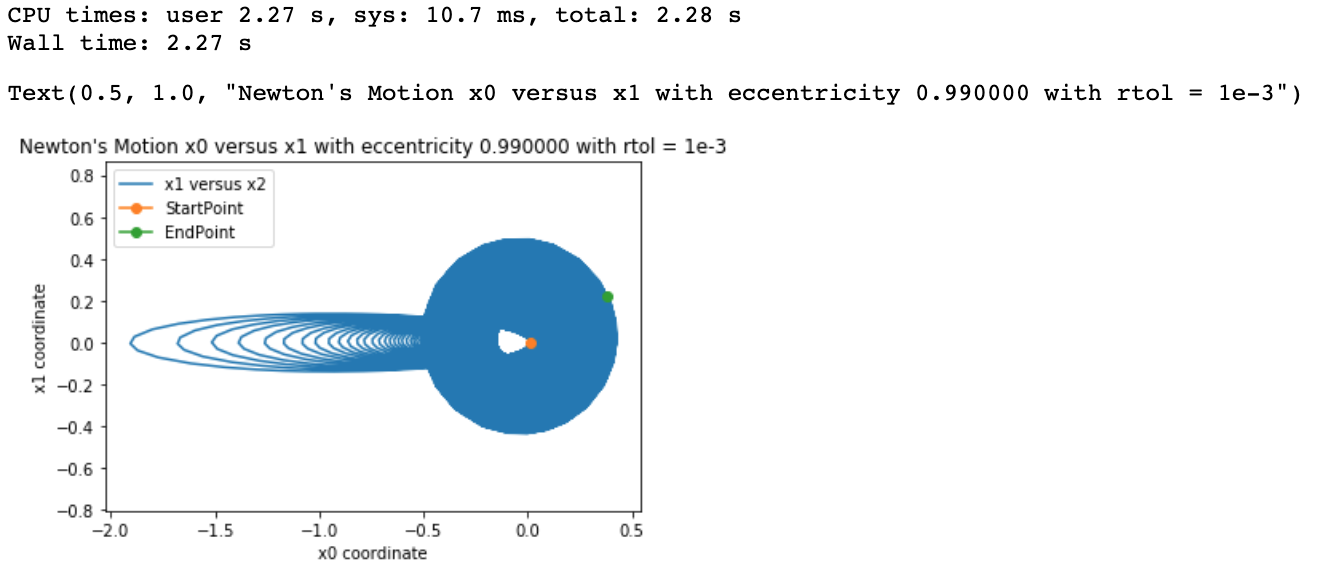
\includegraphics[scale = 0.8]{3}\newpage .\\
tol = -4, it take 7.18s to calculate\\
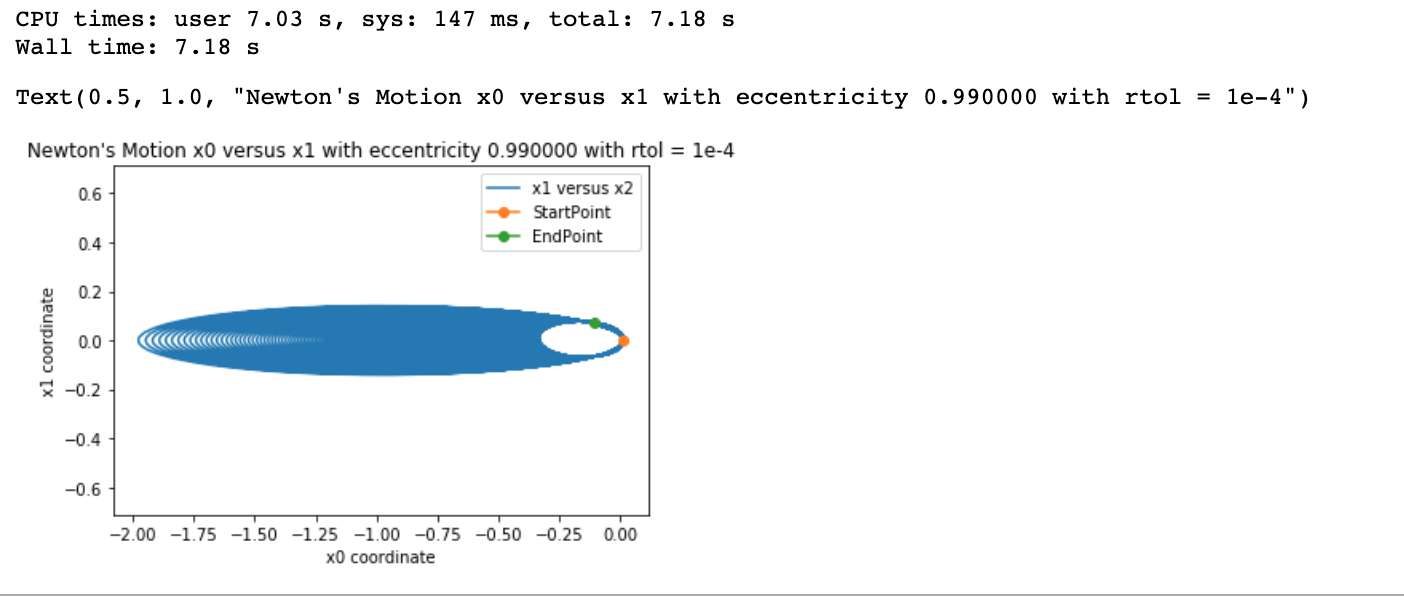
\includegraphics[scale = 0.8]{4}
tol = -5, extremely inaccurate\\
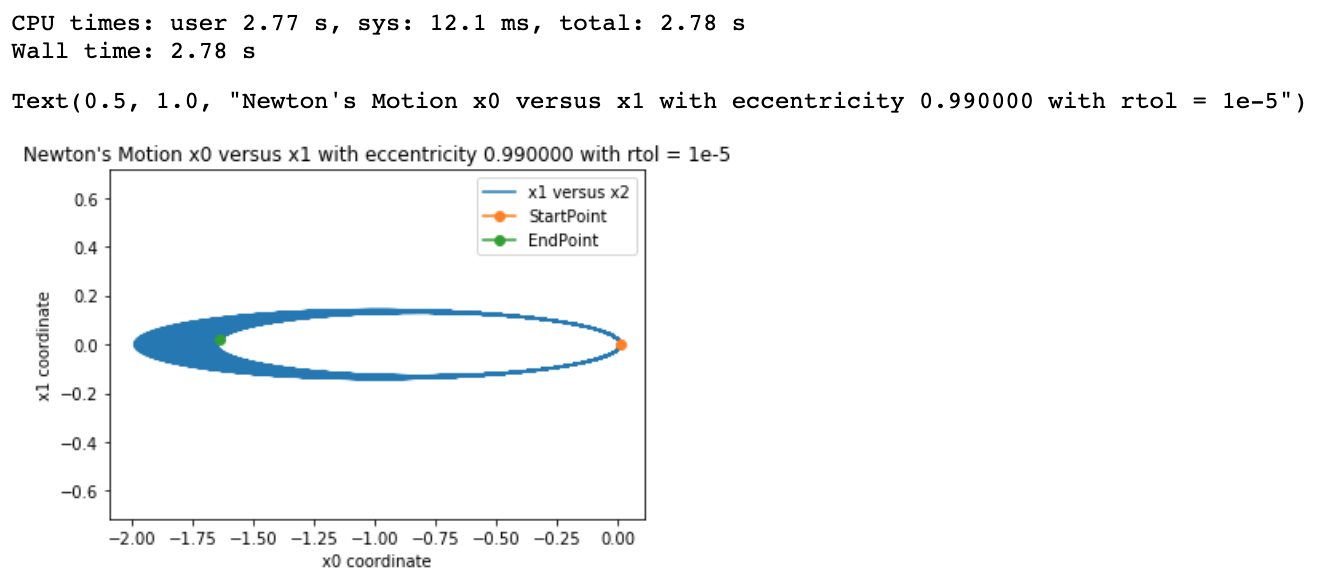
\includegraphics[scale = 0.8]{5}\newpage .\\
tol = -6, more accurate\\
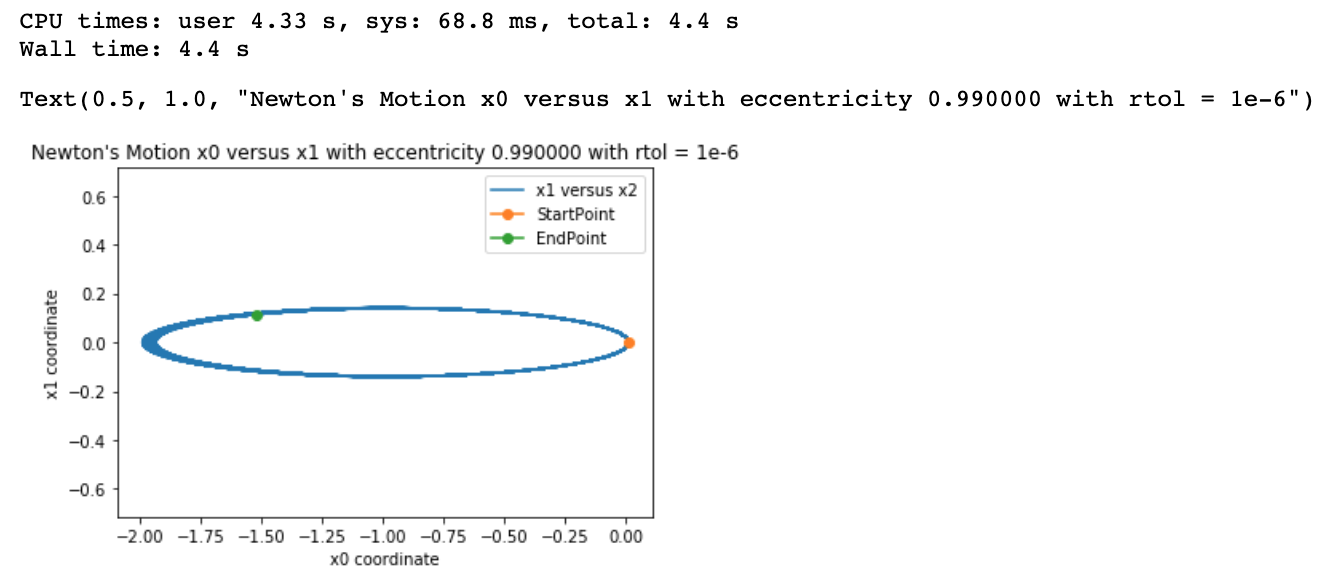
\includegraphics[scale = 0.8]{6}
tol = -7, same, time gradually rise\\
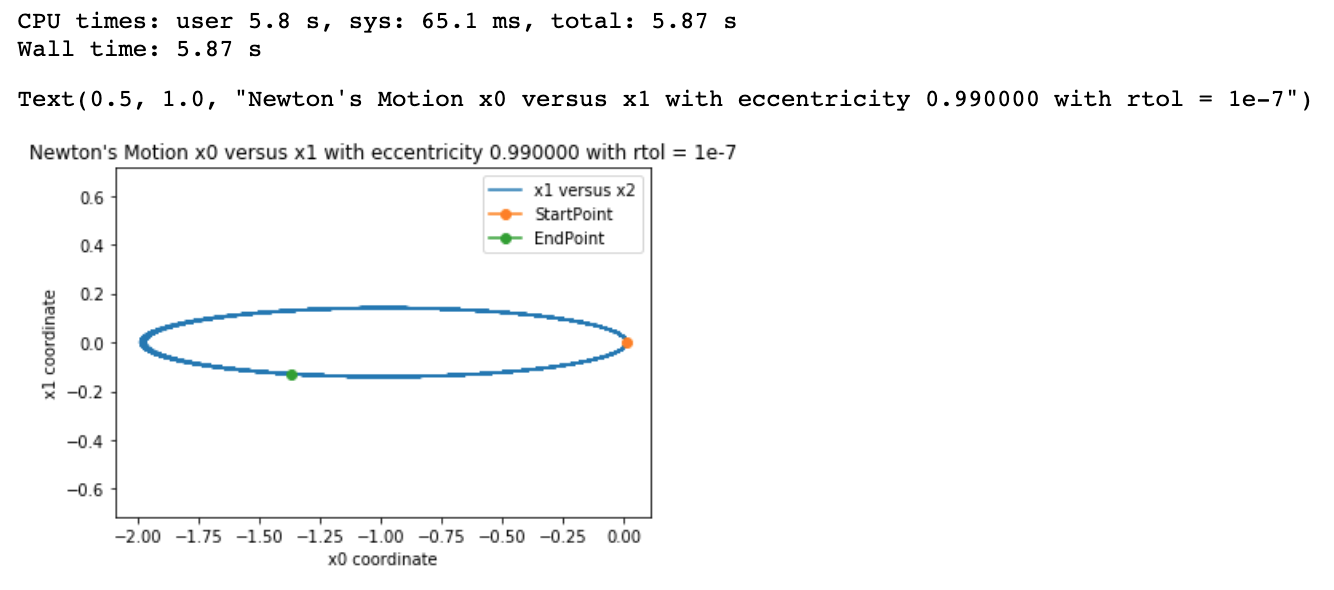
\includegraphics[scale = 0.8]{7.png}\newpage .\\
tol = -8, accuracy grow, running time rise drastically\\
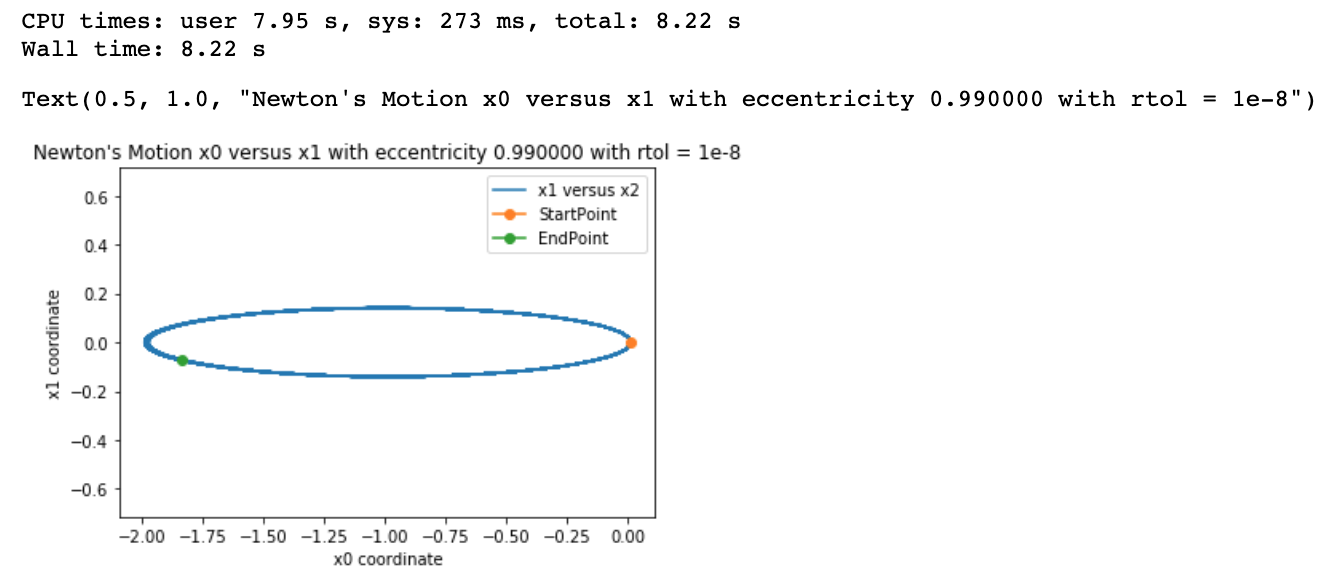
\includegraphics[scale = 0.8]{8}
tol = -9, running time drop slightly\\
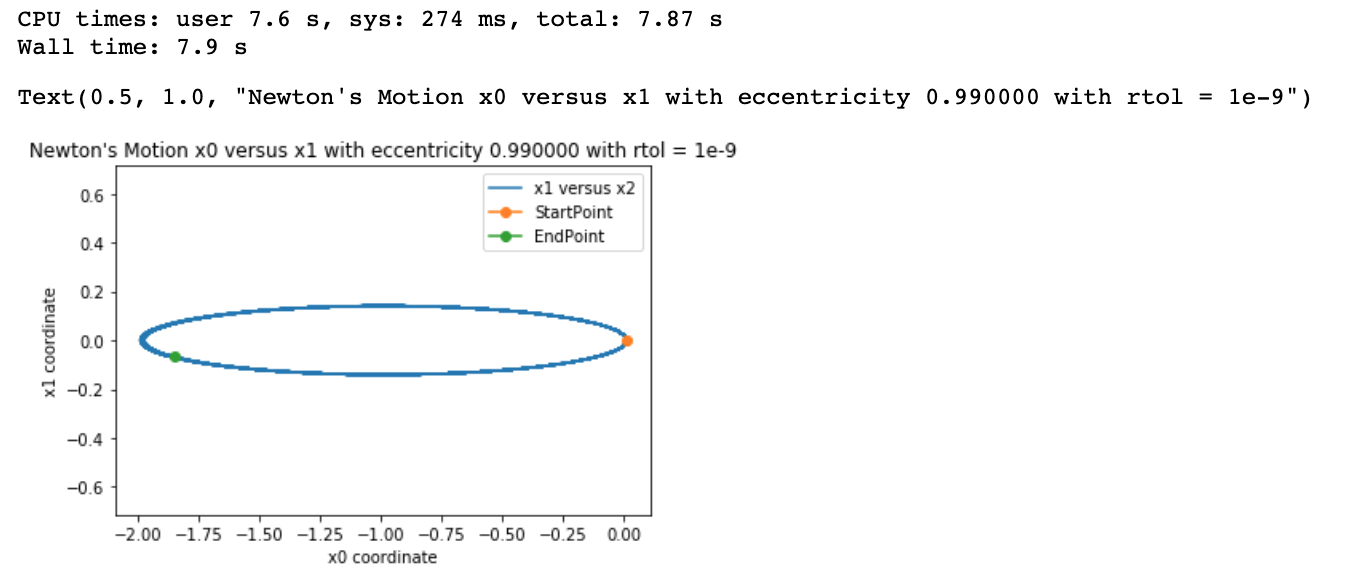
\includegraphics[scale = 0.8]{9.png}\newpage
tol = -10, running drop slightly\\
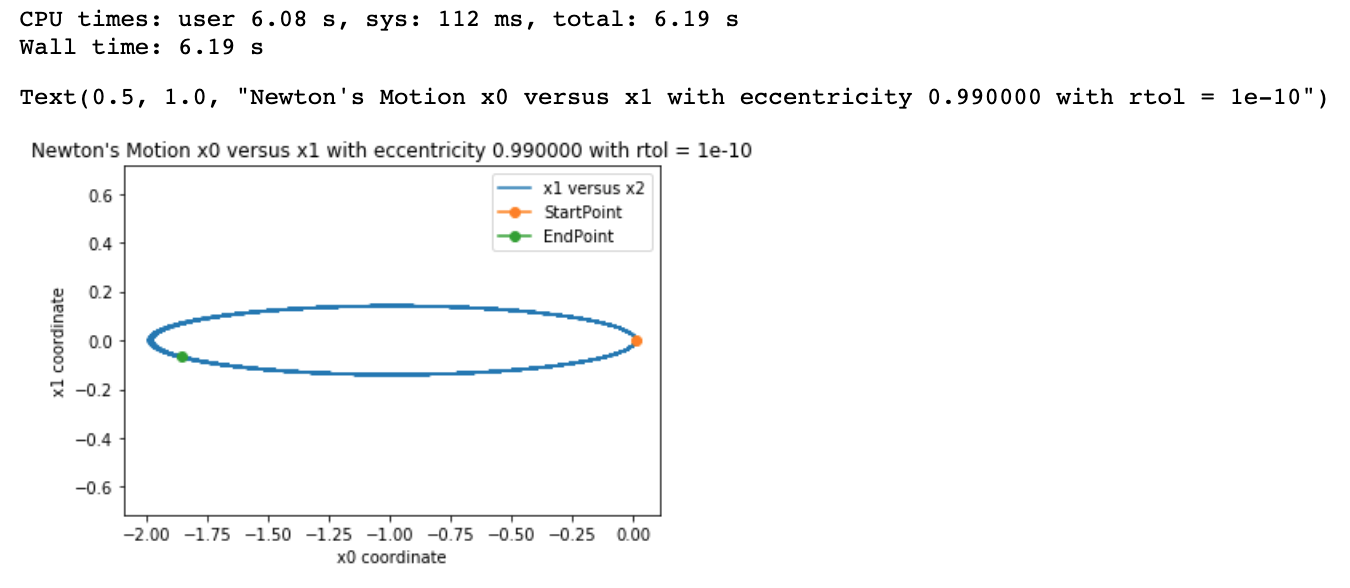
\includegraphics[scale = 0.8]{10.png}
tol = -11, extremely inaccurate\\
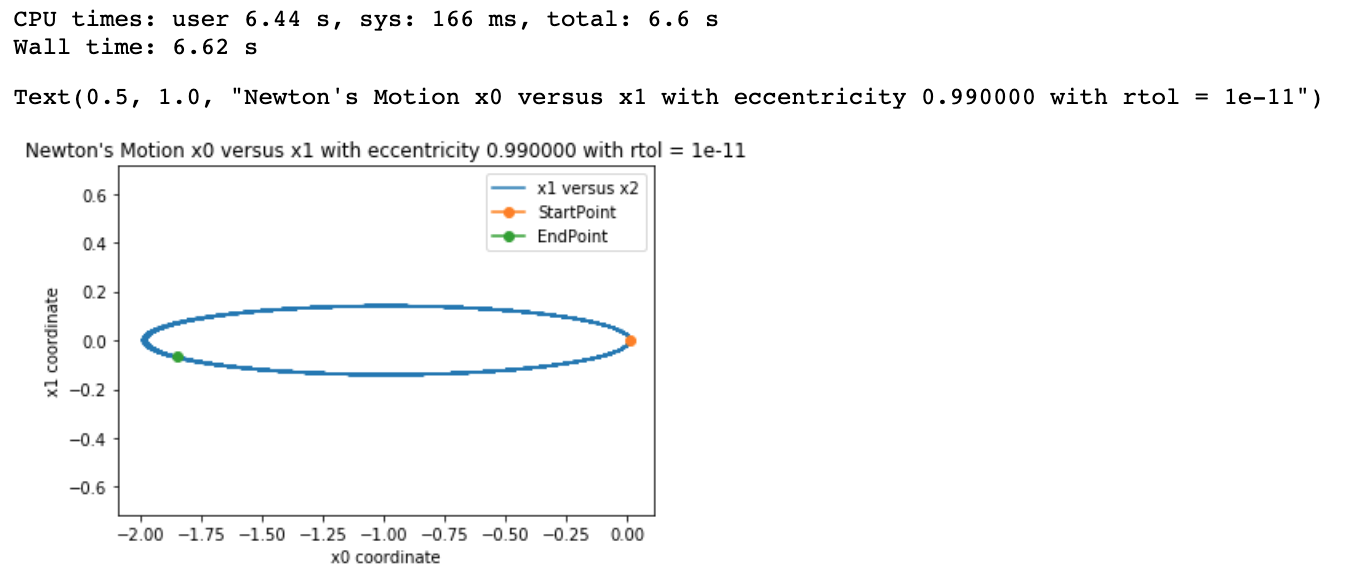
\includegraphics[scale = 0.8]{11.png}\\
Conclusion: (tol = n meaning rtol = $10^{-n}$) in general, running time grows as accuracy gets precise. However, it is not the all situation, in some cases, like tol = 4, tol = 8, their running time get very long. Actually, tol = 4 takes more times than any others tol except 8. in some local area, running time even decrease as tol increase.
	Accuracy is clearly getting better as rtol get smaller. Basing on the observation on the alignment of trajectory. However, the deviation of ending point is inevitable, which maybe related to step size.

\end{document}
